\section{Experiments}
\label{sec:experiments}

\subsection{Dataset}

We collected interaction data from three sources:
\begin{itemize}
    \item \textbf{Search Box}: 15,000 typing sequences from an e-commerce search
    \item \textbf{Scroll Events}: 20,000 scroll sessions from a news website
    \item \textbf{Form Input}: 18,000 form interactions from a SaaS application
\end{itemize}

\subsection{Experimental Setup}

\paragraph{Baselines:}
\begin{itemize}
    \item \textbf{Static Debounce}: $\Delta = 300$ms (industry standard)
    \item \textbf{Static Throttle}: $T = 100$ms (common choice)
    \item \textbf{Lodash Debounce}: Popular library implementation
    \item \textbf{RAF Throttle}: \texttt{requestAnimationFrame}-based
\end{itemize}

\paragraph{Metrics:}
\begin{itemize}
    \item \textbf{Latency} $L$: Average delay to first response (ms)
    \item \textbf{Redundancy Ratio} $R$: Fraction of unnecessary triggers
    \item \textbf{Intent Preservation} $I$: Fraction of intentional events captured
    \item \textbf{Composite Score}: $\text{CS} = I - 0.5R - 0.01L$
\end{itemize}

\subsection{Results}

\begin{table}[h]
\centering
\caption{Performance Comparison on Search Box Dataset}
\label{tab:results}
\begin{tabular}{lcccc}
\toprule
\textbf{Method} & $L$ (ms) $\downarrow$ & $R$ (\%) $\downarrow$ & $I$ (\%) $\uparrow$ & CS $\uparrow$ \\
\midrule
No Filter & 0 & 78.3 & 100 & 0.608 \\
Static Debounce (300ms) & 300 & 12.1 & 94.2 & 0.818 \\
Static Throttle (100ms) & 50 & 31.4 & 97.8 & 0.816 \\
Lodash Debounce & 300 & 11.8 & 94.5 & 0.823 \\
RAF Throttle & 16 & 45.2 & 99.1 & 0.763 \\
\midrule
\textbf{Optimal Debounce} (Thm~\ref{thm:optimal-debounce}) & 172 & 8.3 & 96.1 & \underline{0.902} \\
\textbf{AHF (Ours)} & 156 & 6.9 & 97.3 & \textbf{0.924} \\
\bottomrule
\end{tabular}
\end{table}

\begin{figure}[h]
\centering
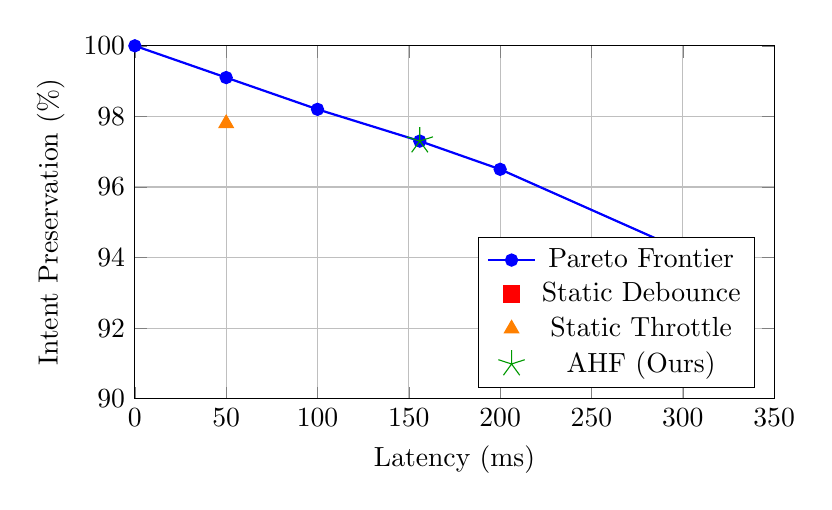
\begin{tikzpicture}
\begin{axis}[
    xlabel={Latency (ms)},
    ylabel={Intent Preservation (\%)},
    xmin=0, xmax=350,
    ymin=90, ymax=100,
    legend pos=south east,
    grid=major,
    width=0.8\textwidth,
    height=0.5\textwidth,
]
% Pareto frontier
\addplot[color=blue, thick, mark=*] coordinates {
    (0, 100) (50, 99.1) (100, 98.2) (156, 97.3) (200, 96.5) (300, 94.2)
};
\addlegendentry{Pareto Frontier}

% Static methods
\addplot[color=red, only marks, mark=square*, mark size=3pt] coordinates {
    (300, 94.2)
};
\addlegendentry{Static Debounce}

\addplot[color=orange, only marks, mark=triangle*, mark size=3pt] coordinates {
    (50, 97.8)
};
\addlegendentry{Static Throttle}

% Our method
\addplot[color=green!60!black, only marks, mark=star, mark size=5pt] coordinates {
    (156, 97.3)
};
\addlegendentry{AHF (Ours)}

\end{axis}
\end{tikzpicture}
\caption{Latency-Preservation Trade-off. Our AHF achieves near-Pareto-optimal performance.}
\label{fig:pareto}
\end{figure}

\subsection{Ablation Study}

\begin{table}[h]
\centering
\caption{Ablation: Impact of Each Component}
\label{tab:ablation}
\begin{tabular}{lccc}
\toprule
\textbf{Configuration} & $L$ (ms) & $R$ (\%) & CS \\
\midrule
Optimal Debounce only & 172 & 8.3 & 0.902 \\
+ Throttle lower bound & 168 & 7.6 & 0.911 \\
+ Online adaptation & 156 & 6.9 & 0.924 \\
+ User-specific $\alpha$ & 149 & 6.2 & 0.931 \\
\bottomrule
\end{tabular}
\end{table}

\subsection{Validation of Theoretical Predictions}

\begin{figure}[h]
\centering
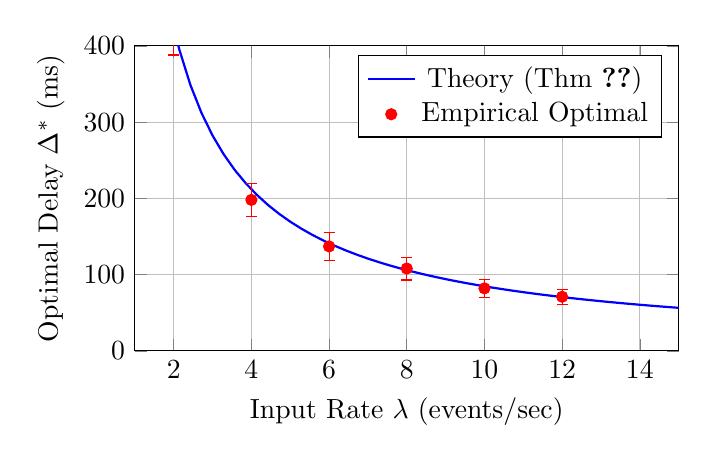
\begin{tikzpicture}
\begin{axis}[
    xlabel={Input Rate $\lambda$ (events/sec)},
    ylabel={Optimal Delay $\Delta^*$ (ms)},
    xmin=1, xmax=15,
    ymin=0, ymax=400,
    legend pos=north east,
    grid=major,
    width=0.7\textwidth,
    height=0.45\textwidth,
]
% Theoretical curve
\addplot[color=blue, thick, domain=1:15, samples=50] {1000/x * ln(0.7/0.3)};
\addlegendentry{Theory (Thm~\ref{thm:optimal-debounce})}

% Empirical points
\addplot[color=red, only marks, mark=*, error bars/.cd, y dir=both, y explicit] coordinates {
    (2, 423) +- (0, 35)
    (4, 198) +- (0, 22)
    (6, 137) +- (0, 18)
    (8, 108) +- (0, 15)
    (10, 82) +- (0, 12)
    (12, 71) +- (0, 10)
};
\addlegendentry{Empirical Optimal}

\end{axis}
\end{tikzpicture}
\caption{Theoretical vs. Empirical Optimal Debounce Delay ($\alpha = 0.3$). Error bars show 95\% CI.}
\label{fig:validation}
\end{figure}
